\documentclass[]{article}
\usepackage{lmodern}
\usepackage{amssymb,amsmath}
\usepackage{ifxetex,ifluatex}
\usepackage{fixltx2e} % provides \textsubscript
\ifnum 0\ifxetex 1\fi\ifluatex 1\fi=0 % if pdftex
  \usepackage[T1]{fontenc}
  \usepackage[utf8]{inputenc}
\else % if luatex or xelatex
  \ifxetex
    \usepackage{mathspec}
  \else
    \usepackage{fontspec}
  \fi
  \defaultfontfeatures{Ligatures=TeX,Scale=MatchLowercase}
  \newcommand{\euro}{€}
\fi
% use upquote if available, for straight quotes in verbatim environments
\IfFileExists{upquote.sty}{\usepackage{upquote}}{}
% use microtype if available
\IfFileExists{microtype.sty}{%
\usepackage{microtype}
\UseMicrotypeSet[protrusion]{basicmath} % disable protrusion for tt fonts
}{}
\usepackage[margin=1in]{geometry}
\usepackage{hyperref}
\PassOptionsToPackage{usenames,dvipsnames}{color} % color is loaded by hyperref
\hypersetup{unicode=true,
            pdftitle={Development of Scholarly Disciplines},
            pdfauthor={Brooks Ambrose},
            pdfborder={0 0 0},
            breaklinks=true}
\urlstyle{same}  % don't use monospace font for urls
\usepackage{longtable,booktabs}
\usepackage{graphicx,grffile}
\makeatletter
\def\maxwidth{\ifdim\Gin@nat@width>\linewidth\linewidth\else\Gin@nat@width\fi}
\def\maxheight{\ifdim\Gin@nat@height>\textheight\textheight\else\Gin@nat@height\fi}
\makeatother
% Scale images if necessary, so that they will not overflow the page
% margins by default, and it is still possible to overwrite the defaults
% using explicit options in \includegraphics[width, height, ...]{}
\setkeys{Gin}{width=\maxwidth,height=\maxheight,keepaspectratio}
\setlength{\parindent}{0pt}
\setlength{\parskip}{6pt plus 2pt minus 1pt}
\setlength{\emergencystretch}{3em}  % prevent overfull lines
\providecommand{\tightlist}{%
  \setlength{\itemsep}{0pt}\setlength{\parskip}{0pt}}
\setcounter{secnumdepth}{0}

%%% Use protect on footnotes to avoid problems with footnotes in titles
\let\rmarkdownfootnote\footnote%
\def\footnote{\protect\rmarkdownfootnote}

%%% Change title format to be more compact
\usepackage{titling}

% Create subtitle command for use in maketitle
\newcommand{\subtitle}[1]{
  \posttitle{
    \begin{center}\large#1\end{center}
    }
}

\setlength{\droptitle}{-2em}
  \title{Development of Scholarly Disciplines}
  \pretitle{\vspace{\droptitle}\centering\huge}
  \posttitle{\par}
  \author{Brooks Ambrose}
  \preauthor{\centering\large\emph}
  \postauthor{\par}
  \predate{\centering\large\emph}
  \postdate{\par}
  \date{October 21, 2015}


\usepackage{dcolumn}

% Redefines (sub)paragraphs to behave more like sections
\ifx\paragraph\undefined\else
\let\oldparagraph\paragraph
\renewcommand{\paragraph}[1]{\oldparagraph{#1}\mbox{}}
\fi
\ifx\subparagraph\undefined\else
\let\oldsubparagraph\subparagraph
\renewcommand{\subparagraph}[1]{\oldsubparagraph{#1}\mbox{}}
\fi

\begin{document}
\maketitle

{
\setcounter{tocdepth}{2}
\tableofcontents
}
\section{References and the Development of Scholarly Disciplines
(900)}\label{references-and-the-development-of-scholarly-disciplines-900}

Between 1900 and 1925 each American social science discipline
distinguished itself as an autonomous profession. .

A key component of the establishment of each as a field was the
development of a pan-disciplinary convention of citing references. We
take for granted the use of citations as a currency of information flow
and authorial recognition, but early in the century it was not a norm to
provide precisely codified descriptions of consulted publications.
Citations were often very casual, referencing an author by title and
surname only, and referring to an idea and not any work in particular. .
These proto-citations required a contemporary grasp of context to be
intelligible, as do citations today, but they lacked the address-like
codification that would allow the unknowing reader to actually locate
the source in question.

Over several decades however the act of referencing became both more
common and more consistently codified. Whereas in 1900 the average
number of references in an article bibliography for the journal
\textless{}\textgreater{} was \textless{}\textgreater{}, by 1925 it had
grown to \textless{}\textgreater{} and by 1940 to
\textless{}\textgreater{}.

These references indicate the general technical upgrading of scholarly
rigor. Scholars were, especially among peers, expected to be transparent
about their influences, to be deferent to their predecessors and fair to
their opponents, and to provide readers with the means to follow up on
claims made about sources.

But what had scholars been doing previously if not scholarship? If
disciplinary conventions were not solid, was their work undisciplined?
The answers are not merely semantic; they involve the task of
disentangling the relationship between two very different aspects of
creative occupations. On one hand, scholars have always struggled to
make sense in public about what they have struggled to make sense of in
private. However we conceptualize the basis of thought and expression,
internal and external representations are ontologically distinct
processes and the mechanisms of translation between them are
nontrivially constructed and maintained. What distinguishes early
scholars from the inheritors of their craft is a difference of
proportion between internal and external requirements; beset by a
smaller and less powerful audience early scholars were more free to
engage in idiosyncrasy, to commit their energy to an internal struggle
of making sense of their own ideas and those cast in front of them. This
did not mean that they worked in isolation; insofar as they were
required to meet heteronomous standards these were content standards,
either defined by peer pressure, by the personal relationships of
rivalry and comraderie (c.f. restricted fields of cultural production
{[}\href{mailto:/@Bourdieu}{\nolinkurl{/@Bourdieu}}:1993vo/ :39{]}) or
by the tastes of lay audiences who mattered for the scholar's
livelihood.

The relationships defining these content standards were institutions
like any other mechanisms restricting what scholars might otherwise do
if left alone. However they were not disciplinary standards. Adherence
to them did not signal membership in the profession of scholarship.
Instead content standards signaled their intellectual location directly;
recognizing scholars required understanding the content of what they
were speaking.

As scholarship grew in published work and personnel, references also
became a sign of dependence, since one scholar could not be expected to
master more than a component of her milieu.

References then constitute an important element of not only scholarly
practice, but after a period of institutional development, scholarly
orthopraxy. It is only in the narrowest sense of a subfield that
normativity can be characterized as a form of orthodoxy, or correct
thought. The normative power of a profession can at best be a form of
correct practice that puts only very weak restrictions on correct
cultural or intellectual content. But differently, two scholars on equal
footing may consider each other's substantive work profane, but this
mere fact of heterodoxy would not normally disqualify either of them
from membership in the profession. The submission of an
``unprofessional'' manuscript, one that, for instance, did not adhere to
citation conventions, would bar the work from publication.

Scholarship then is a cultural lifeworld steered by a professional
system {[}@Habermas:1987{]}. Habermas's concepts provide a more precise
forumulation of the familar embeddeness concept in sociology. The
metaphorical content of embeddeness suggests close contact between the
focal field of practice and the more or less hidden mechanisms that
support it. However, these supporting mechanisms often stand at arms
length from the practices of, for instance, scholarly discourse. If we
presume that scholarly discourse is exemplifed by verbal exchanges, for
instance, among students in a seminar or symposium, between a reader and
the written words of a reference, or between a writer and her own
consciousness, then by mechanisms of discourse we must mean the ways
that proximate utterances shape their antecedeants in streams of
discourse @CA, @CommunitiesOfPractice, @Wittgenstein{]}. Professions
then are embedded much like pylons struck into the shifting sands of
language. However this reverses the embeddeness metaphor. Scholarly
discourse is not supported by the unseen mechanisms of the profession,
rather the profession is supported by the unseen mechanisms of the
discourse. Without the churn of language and thought, editors and
reviewers would have no content to split and bolster, and no audience to
serve the cream to. We might say that system and lifeworld have an
epigenetic relationship. However what we are uncovering here is not the
hierarchy between professions and culture, but the lack thereof.
Professions and culture are interpenetrating; the resources and chance
opportunities determining one's control over the other turnover to such
an extent that we might as well accept Sewell's anti theory of
structural multiplicity @Sewell?:{]}.

Abbott calls culture or lifeworld an interactional field. Cf abbots
basketweave

@Abbott:2001uy{]}

\subsection{Paradigms, Structural Mechanisms, and Stage-sequential
Development}\label{paradigms-structural-mechanisms-and-stage-sequential-development}

It is the contention of this study that this transition in scholarly
practice between casual and informal citation behavior is both a cause
and a consequence of a developmental transition in the social an
cultural structures of scholarly fields.

A substantive theory of such structures was introduced by Kuhn in the
\emph{The Structure of Scientific Revolutions} {[}-@Kuhn:1970vn{]}.
Rather than reproducing Kuhn's theory, my aim here is to generalize his
model--which was intended for application to the natural sciences
especially prior to the maturation of the university system in the
twentieth century--to scholarship in general, in the United States, and
in the first half of the twentieth century. Though my theoretical scope
aims to be inclusive all disciplines finding a support in the U.S.
university system, I will restrict my empirical investigations to
selected disciplines in the social sciences.

To generalize Kuhn I draw on more recent work in the sociologies of
knowledge, of cultural production, and of professions. Whereas Kuhn
focused intently on three relationships, of scientists to paradigmatic
works, to their peer scientists in the narrowest sense, and to their own
direct labor of scientists to

Citation practices however did not necessarily represent better
scholarly practice, in the sense of a capacity to communicate more
clearly and with fewer errors of fact or interpretation. These different
possible meanings of a reference made them polysemic in a way that
belied a ``disciplined'' discourse. Rather than trying to ``get Kuhn
right'', I will draw selectively to fill out the conceptual matrix
outlined below.

A lacuna in Kuhn's model of scientific development concerns a clear
conceptual model of what might be called non-cyclical or
original/genetic development. The basic cyclical pattern is between
revolutionary and normal science, where each is always a prerequisite
for the other. This poses a chicken and egg question; presumably a
different process explains an ``original'' revolution developing out of
no prior paradigm. Kuhn is able to forestall this question through an
historical approach where antecedent moments in historical (not
analytical) development are always at hand for the researcher who has
done her homework.

\subsubsection{Kuhn's uses of the term}\label{kuhns-uses-of-the-term}

\subsubsection{A reconceptualization}\label{a-reconceptualization}

Paradigm has at least two referents, one concerning the process of
cultural production which emphasizes the relationship of creators to
their craft, and the other concerning the normative regimes within the
community of craftspeople. The cultural reference is embedded in the
eytemology of the term; a paradigm is a prototypical cultural product
that serves as a model or basis of comparison for the reproduction and
extension of knowledge, either that gleaned from the lesson of the
object or knolwedge about the process of creation. Not all objects are
good paradigms in this sense; a paradigm has staying power if it poses
problems without answering them, and if the solutions are partially but
not fully explicated.

The pattern of oscillation between normal and revolutionary science in
Kuhnian theory can be thought of as recurring moments in the continuous
development of a stable thing (professional science), or it can treated
as a very simple ecological model with only two things (rival paradigms)
drawing on the same scarce resource base (professional science).

In the sociology of music a very different developmental theory has been
proposed centering on the concept of genre {[}-@Lena:2008er{]}. Genres
differ significantly from paradigms in that they do not require a strong
cultural consensus to be reproduced. Disparate cultural objects and
practices may be united under a genre if similarities are successfully
socially constructed. While genre classifications may become normative
they are usually difficult to enforce; exogenous pressure is usually
required to condemn something as violate. This is because genre
inclusion tends to occur when a threshold of similarity is crossed by,
so to speak, checking of enough boxes on a checklist of attributes,
while remaining unclassified features of the object are ignorable if a
preponderance evidence in favor of inclusion is established.

Not so with paradigms; a novel object must be thoroughly vetted to be
considered relevant to the cause of normal science. If it does not pass
a sniff test it will be ignored, and if it insists on being recognized
and remains incommensurate with extant expectations then the familiar
revolutionary crisis ensues.

\subsection{Mechanisms}\label{mechanisms}

\begin{table}[!htbp] \centering 
  \caption{Ontology} 
  \label{} 
\begin{tabular}{@{\extracolsep{5pt}} ccc} 
\\[-1.8ex]\hline 
\hline \\[-1.8ex] 
 & Cultural & Social \\ 
\hline \\[-1.8ex] 
Micro & a & c \\ 
Macro & b & d \\ 
\hline \\[-1.8ex] 
\end{tabular} 
\end{table}

\begin{figure}[htbp]
\centering

\includegraphics{/Users/bambrose/Dropbox/GitHub/manuscripts/Figs/ch0/sensemaking.pdf}
\caption{Sensemaking entails discriminating first between relevent and
irrelevant material, and second between relevant and productive
resources.}
\end{figure}

Struggles to establish disciplines as professions were hard fought,
harder still because each was a contest on cultural, cognitive, and
social fronts. While all human behavior can be analyzed as consisting in
different ratios of all three components, the institutional development
of professions procedes in a conditional order.

In sociology to declare something an institution is to ask how patterns
of human behavior became regular and to excavate the hidden mechanisms
that maintain that regularity within limits. Religious practice is
regulated by the church, political practice by the state
{[}@Sewell:2005vq\textbackslash{}:172{]}. Such large scale organizations
eclipse the cultures that provide the content around which they
initially organized. They assure their own cultural inputs, and may be
open or closed with respect to novel culture.

Paradigms reflect an advanced stage of institutional development in the
history of disciplines. They presuppose professions, which provide the
organizational resources necessary to enforce conventions. Though
paradigms are often associated with ideas.

Culture preceeds cognition in the sense that practices develop tacitly
before they are ``recognized'' explicitly, and indeed recognition is,
while often transformative, not actually necessary. On the contrary a
cultural thing, whether an object or a practice, must already exist for
it to be recognized. Likewise cognition, especially classification,
preceeds social control Cultural processes center on human interaction
with meaningfully constituted objects. This far reaching concept is
usefully characterized in the tradition of Geertz where culture exists
at the intersection of symbolically organized thought and concrete
practice. Since Geertz priority has been placed This polarity between
real and ideal may be adapted in a tr

A discipline must cohere culturally before it can professionalize, and
this process occurs in four stages. First, a prototypical set of
productions--articles, books and lectures--had either to be found or
invented, and the patterns they established had to be reproduced without
the benefits of consistent resources or conventions. Second, assembeled
productions had to become recognizable; they had to be labeled and
grouped together according to a consistent symbolism, and that symbolism
had to be learned within a broader milieu. Third, after a symbolic index
could be taken for granted, disciplines would be stillborn if they could
not maintain productivity. Would-be disciples had to produce enough new
material to support an audience intially of peers and then of larger
publics. Fourth, to emerge as professions, disciples had to have a
reasonable chance of being awarded scarce resources within the academy.
The ability to attach the disciplinary label to departments and
professorships marked the beginning of a viable adolescence. If a
discipline could aqcuire the machinery of education it could control the
presumption of its own legitimacy, at least among new generations of
students.

\begin{table}[!htbp]
  \centering
  \caption{Mechanisms Operating at each Stage of Development}
  \label{}
\begin{tabular}{@{\extracolsep{5pt}}llll}
\\[-1.8ex] \hline \\[-1.8ex] 
          & \multicolumn{3}{c}{Stage}                                       \\ \\[-1.8ex] \cline{2-4} \\[-1.8ex]
Mechanism & Aparadigmatic & Preparadigmatic & Paradigmatic \\ \\[-1.8ex] \hline \\[-1.8ex]
Cultural  & Charisma \cite{Gustin:1973ul}      & Genre           & Paradigm     \\
Cognitive & Chaos         & Schema          & Schema       \\
Social    & Autonomy      & Heteronomy      & Heteronomy   \\ \\[-1.8ex] \hline \\[-1.8ex]
\multicolumn{4}{l}{}                                                       
\end{tabular}
\end{table}

This study is about the second stage of development, recognition. I
assume that protoypes of disciplinary knowledge were readily available
in the United States by the end of the 19th century, and that the
challenge for disciples was to relabel what had already been
accomplished in an effort to create an occupation out of what was
formally a personal undertaking, an obsession or a pastime.

\subsubsection{Cultural Sensemaking}\label{cultural-sensemaking}

In order to regulate their own creative activity, disciples curated
prototypes into sets that drew a boundary, however roughly, around the
tacit definition of what they thought they were doing. These acts of
sorting allowed prototypes to be organized without requiring the
organizer to explain the rules of their order.

Wherever personal sets overlapped the intersection would form a smaller
set of higher status. This tendency to overlap one's personal cultural
toolkit with that of others was a form of deference to peers as well as
to common culture. This allowed disciples, without necessarily
intending, to both claim membership in the discipline and indulge in
their idiosyncratic variations on the essence of the discipline. Indeed
idiosyncrasy would be tolerable only to the extent that a scholar could
in the same breath genuflect to what was already understood.

While new references to the overlapping set reinforced its status they
also winnowed its content. Paradoxically by begging to peers that they
recognize some novel prototype scholars would have to also pay homage to
the core. They could not then elevate their own interests above that of
the growing stock of taken for granted knowledge, since introducing
something could not garner attention without attaching it to something
old.

\begin{figure}[htbp]
\centering

\includegraphics{/Users/bambrose/Dropbox/GitHub/manuscripts/Figs/ch0/sensemaking.pdf}
\caption{Sensemaking entails discriminating first between relevent and
irrelevant material, and second between relevant and productive
resources.}
\end{figure}

The rejoinder to the claim that nothing can overtake the core is found
in Kuhnian accounts of scientific revolution. Yet the theory of
referential coherence could not be further from that of paradigmatic
coherence. The great advantage of using references as the currency of
disciplinary communication and exchange is that their meanings can be
assumed, and the inevitable disagreements over interpretation can be
easily ignored so long as conversation floats just above matters of
substance. Paradigmatic agreement is not culturally, that is
autonomously, possible unless one makes a very strong empirical
convergence assumption. Exogenous reality must weigh so heavily on the
mind that the concept of interpretation can be dismissed. If however
interpretive variation is the norm then we can also posit that within
limits the same larder satisfies many chefs so long as each is free to
cook according to her particular tastes.

Such tastes are not merely metaphorical; an important feature of this
conceptualization is that scholars produce work for their own
consumption first, especially early in the development of a discipline.
There must be a point of origin where cultural sensemaking is
idiosyncratic to the creator. It is only with time that multiple
idiosyncracies can be commensurated, and given such commensuration there
can be no expectation that consensus develops to the point of uniformity
in thought even in a solitary thinker not to mention a community of
scholars.

If cultural sensemaking were the only mechanism of disciplinary
coherence then it would draw people together but only weakly. Though the
kernel of a core set of references may grow this does not imply a
tendency for disciplines to become closed culturally. What truly bonds
scholars is the opportunity to stand up and be seen through ceremonies
around the core while being otherwise totally invisible when pursuing
idiosyncratic interests.

\subsubsection{Relevance}\label{relevance}

\begin{longtable}[c]{@{}lll@{}}
\toprule
& irregular & regular\tabularnewline
\midrule
\endhead
include & retroject & retroject\tabularnewline
tend & object & object\tabularnewline
exclude & reject & abject\tabularnewline
\bottomrule
\end{longtable}

\subsubsection{Cognition}\label{cognition}

Here I attempt to combine internalist and externalist theories of
culture. ``Art for art's sake'' characterizes the internalist view;
cultural expression is both motivated and regulated by a concept of the
object and standards of quality that, no matter how they got there, are
autonomously held in the mind of the creator. ``Art for the artists's
sake'' characterizes the externalist view, where the interests of the
creator may be multiply determined by a number of social pressures
including fame, fortune, fraud, or force. Many couplets of opposing
forces--knowledge and professions, culture and society, truth and
power--merely replicate this basic distinction.

Yet the internal/external distinction is generic and restrictive. The
underlying references concern how a person might orient herself to
cultural production, and how such productive activity may be embedded in
larger social structures and cultural milieus. I break this distinction
into three simple processes that make creative work easier.

\subsubsection{Social Structures}\label{social-structures}

It is during the period where recognition develops that social control
begins to collide with personal sensemaking. This control may at first
go no further than a group of peers beginning to enforce conventions of
practice or symbolism by asking or demanding that a concept be manifest
in this way and not that way, or that it not be expressed at all. If the
chief mode of personal sensemaking is sorting objects into sets of
similarity or difference, the nascent form of social intrusion on
cultural sensemaking is attaching labels to the sets of others. If a
sensemaker is exposed to sets with the same label and different contents
then any attending pressure of contradiction would be most easily
resolved by direct interference with someone else's process of personal
sensemaking. Disengaging from the contradiction is certainly an option,
but it is likely that the dopplegangers would find themselvs at odds
again if they inhabit the same milieu.

If there is a weak social force drawing thinkers together at the overlap
of their sensemaking, it will pale in comparison to exogenous sources of
social control that can define cultural relevance by fiat, force, fame,
or facilitation.

Even politically motivated ideologies require constant social control to
combat the drift in personal sensemaking.

If a person seeks out social control over their own sensemaking then
they are thoroughly socialized. This tautology may describe some people
most of the time and everyone some of the time. Even if I stipulate that
a sensemaker is delighted when someone else expresses a thought that
makes sense to her, such delight must be predecated on the prior
development of recognition, or else identical thoughts would pass each
other unrecognized like ships in the night.

A cartographic metaphor will be useful. The indexing of the set occurs
when a set is labeled, and this is analogous to the name of a contiguous
territory on a map. The territory is defined only by the boundary that
encloses it, and no knowledge of its contents is necessary to refer to
the label. Any content discovered must be categorized de novo, and the
boundaries provide the decision rule to accomplish this. Recognition of
bounded content occurs when the content is given an address. The address
need only lead a searcher to a point of contact with the content, for
the address is only a reference and bears no knowledge of its own.

It is entirely possible that discourse around a set of references can be
sustained without ever referring to underlying content. The great
efficacy of organizing cultural objects into sets of addresses is that
it is much easier to agree on the address than it is to agree on the
character of what is addressed.

In Parsons's terms the addresses are a form of influence. Influence is a
currency bearing social status that allows communication to occur
generically and at a pace faster than would be the case if the real
underlying content had to be mobilized. Money is the archtypical form of
generalized media, allowing exchanges can be defined prior to the actual
mobilization of goods and services.

By organizing cultural history into categories, disciples solved two
important problems. First, they sanctioned ignorance; lack of knowledge
beyond the curated set would be no threat to disciplinary credentials.
Second, they created a method of communicating tacit knowledge where
formal codification or training was absent. If a scholar were able to
reference the contents of a curated set in ongoing conversations he
would be rewarded with membership in a self-organized community of
scholars including anyone willing to uphold the legitimacy of the
discipline. While variations in the quantity and quality of set
references confer differences in status iternally, a reference no matter
how controversial signaled deference to the discipline and would be
treated as a credential for membership.

Such curation served as a critical factor to scholarly production in
both of its forms, research and education. The cultural artifacts of
curation left by research were the footnotes and bibliographies of books
and articles, that left by education were lectures and course syllabi.

Professional activity routinizing the reproduction of the pattern these
protypes established. They developed legitimacy for the low level of
extant cultural production, low relative to the subsequent historical
growth of disciplines.

Recognition, a process that amounts to the social organization of
existing cultural material. This is the process of genre formation.
Though the term is sometimes use to refer to the entire developing art
world or field of cultural production {[}@Lena:2008er{]}, \emph{genre}
is better reserved to refer to the development of the cognitive
institution alone. Here genres represent the collision of social
constraints with cultural production. \footnote{In Habermas's terms,
  genres represent a development of system against lifeworld. In
  Bourdieu's terms, genres are fields, specifically the definition of
  positions to be taken.} The initial symbols were indexical, allowing
productions to be labeled according to a cogntive categories
representing the disciplines. For the U.S. social sciences, by the end
of the ninteenth century symbolism had already been developed around the
. In this regard scholarly disciplines behave according to a logic of
development that has been articulated in the context of artistic genre.

Tendencies leading to each of these thresholds followed different yet
often intersecting developmental logics.

\subsection{Typology of Relationships}\label{typology-of-relationships}

\begin{longtable}[c]{@{}llll@{}}
\toprule
& super & par & sub\tabularnewline
\midrule
\endhead
super & contest & challenge & subject\tabularnewline
par & challenge & citizen &\tabularnewline
sub & subject & & genteel\tabularnewline
\bottomrule
\end{longtable}

\section{Empirical Foundations (1800)}\label{empirical-foundations-1800}

This brief foray into the different sociocultural functions of citations
may be demonstrated by the observation of the formative moments of U.S.
social science. The impressions left by the earliest social scientists
became a terrain of disciplines and \texttt{try(onm\$sd)} that could be
landscaped but not easily turned over by future generations. Paradigms
or hegemonic cultures developed in the first half of the 20th century.
These paradigms endured even during times of social upheaval such as the
Great Depression and WWII. However, at the dawn of the 1960s, such
monoliths were toppled in quick succession. For the first time in
American history, the cultural heritage was treated in an a la carte
fashion by new generations.

What was really different about the 1960s?

\subsection{Study 1: Labels: Diffusion of Disciplinary
Prefix}\label{study-1-labels-diffusion-of-disciplinary-prefix}

There may not be a formative moment for disciplines, but there are
tendencies of development that when compared are relatively large times
scales show transitions into institutional relationships. Nothing
forbids creators from inventing knoweldge about the world before it is
clear how to label that knowledge. The organization of one's work along
disciplinary lines does however tend to make one more productive.
Audience and contemporary may become obvious, and paths of influence may
present themselves as stimulating creative opportunities. Ultimately
disciplines intersect with organizational resources, first as a market
for tutorship and ultimately as a professorship (c.f. Weber's
description of prebends
{[}\href{mailto:/@Weber}{\nolinkurl{/@Weber}}:1917wi/:343{]}). The
development of such social structures is necessarily endogenous to the
recognition of particular forms of cultural production as belonging to a
category.

Categories then are not the foundation of institutionalizations, but
rather they serve as a hinge between cultural and social phases of
institutional development. In real historical situations an author
cannot wait for her chosen obsession to become institutionalized, and
indeed the likilihood of this happening for her is slim given the rate
of cultural survival. On the contrary she will try to master whatever
extant opportunities exist, then using the traditional production as a
security base, delve into her idiosyncratic persuit with whatever
resources are left over. The stereotype of the artists who suffers for
her craft and dies young and consumed by her obsession is the exception
that proves the rule. What is more likely is a shifting of resource
deployment, first with an investment in the aqcuisition of an income
generating activity and secondly with a shift of attention to the
obsession for as long as neglect of the day job can be tolerated.

What interests us presently is to trace the development of scholarly
disciplines back to a point where they were weakly recognized even if
they were already culturally prolific. We submit that recognition is
empirically identifiable if there exists a flag around which
categorizing coalesces. Categorization can be said to completed when the
set of possible labels for the same cultural object shrinks to a short
and ranked list. The position at the top of that list will be occupied
by what we call the disciplinary prefix, and below it variations on
nouns used to capture different aspects of cultrual content from created
work to the authors themselves.

Consider four social science disciplines--anthropology, economics,
psychology, and sociology. In english the flag uniting the concept of
discipline are the prefixes anth-, econ-, psyc-, and soci-. We contend
that these prefixes will diffuse first as generic and weakly categorical
terms ()

\begin{table}[!htbp] \centering 
  \caption{Flagbearers} 
  \label{} 
\begin{tabular}{@{\extracolsep{5pt}} llll} 
\\[-1.8ex]\hline 
\hline \\[-1.8ex] 
stem & cat & Phrase & N \\ 
\hline \\[-1.8ex] 
anth & 1generic & cultural & $139$ \\ 
anth &  & anthropic & $139$ \\ 
anth & 2discipline & anthropology & $139$ \\ 
anth & 3technical & anthropological & $139$ \\ 
anth & 4profession & anthropologist & $139$ \\ 
econ & 1generic & economic & $139$ \\ 
econ & 2discipline & economics & $139$ \\ 
econ & 3technical & economical & $139$ \\ 
econ & 4profession & economist & $139$ \\ 
poli & 1generic & political & $139$ \\ 
poli & 2discipline & political science & $139$ \\ 
poli & 4profession & political scientist & $139$ \\ 
psyc & 1generic & mental & $139$ \\ 
psyc & 2discipline & psychology & $139$ \\ 
psyc & 3technical & psychological & $139$ \\ 
psyc & 4profession & psychologist & $139$ \\ 
soci & 1generic & social & $139$ \\ 
soci & 2discipline & sociology & $139$ \\ 
soci & 3technical & sociological & $139$ \\ 
soci & 4profession & sociologist & $139$ \\ 
\hline \\[-1.8ex] 
\end{tabular} 
\end{table}

\begin{figure}

{\centering 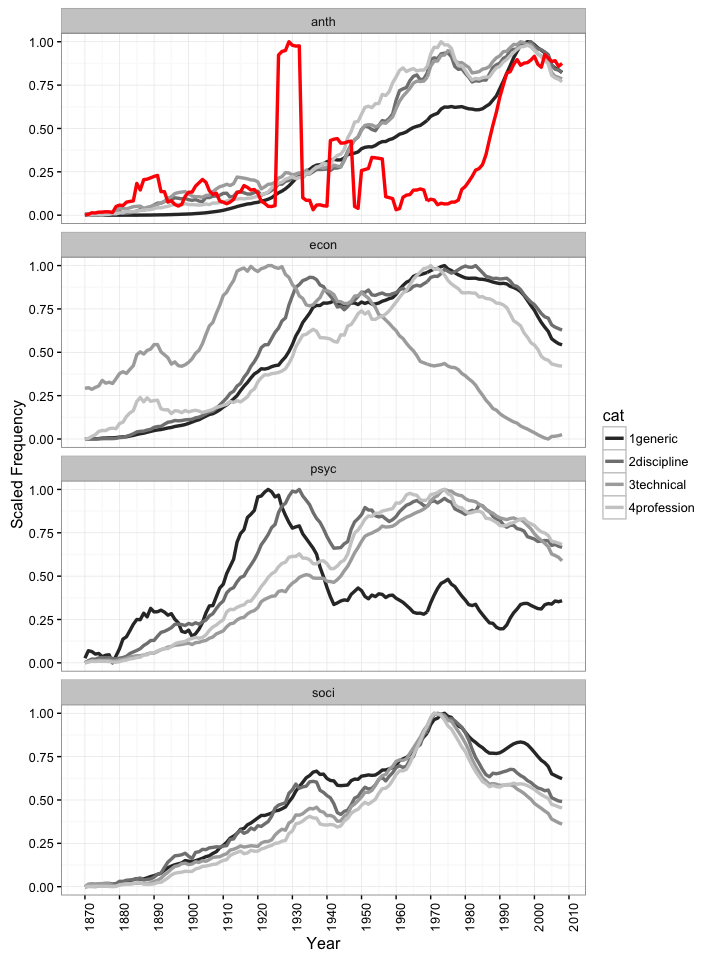
\includegraphics{d2016-ch1_files/figure-latex/f-disciplines-1} 

}

\caption{Disciplinary Prefixes}\label{fig:f-disciplines}
\end{figure}

\subsection{A lexical sample}\label{a-lexical-sample}

The source data are observations on documents spanning years.

Each study depends on a database of records of the contents of journals.
This database is compiled from two sources, JSTOR and the Thompson
Reuters Web of Knowledge Social Science Citation Index (WOK).

Ideally, I would analyze the entire stock of recorded publication
material to give the best chance of observing when authors contravene
institutional boundaries. Practically, I must take a sample, however
sampled networks are not small versions of the population network
{[}@Handcock:2010iw{]}. Sampling may have the effect of degrading the
network cohesion on which community detection methods depend, such that
a method will not detect the same boundaries in a sample as it would in
the population. To avoid a sampling effect on network cohesion, I draw a
full census of articles, reviews, and book reviews from each journal
selected.

Sampling on journals creates another problem, which is to merely
reproduce boundaries coextensive with the journals from which the
articles are drawn. Even though journals market themselves at catering
to particular disciplines and subfields, I should not assume that
authors, editors, and reviewers always obey these distinctions. If a
scholarly field exists with a grounding in two or more journals, the
omission of one may also degrade its cohesion to the point of rendering
its boundaries undetectable. As an indicator of affiliation among
journals, I use Leydesdorff's {[}-@Leydesdorff:2010ci{]}

I should also expect to observe boundaries due to several other
institutional levels higher than journals, like publishers, disciplines,
or national and language groups. To provide ample opportunity to observe
boundaries existing in the space between journals and between academic
disciplines, I also take a large sample of journals

To observe some of these high level institutions, I draw sets of
journals from four social science disciplines--anthropology, sociology,
economics, and political science--and I draw these in blocks from the
same publisher. Journals were selected from the disciplinary
affiliations signaled in their titles. From a JSTOR master list of
archived materials, journals were selected if they contained any of the
disciplinary prefixes anth-, soci-, econ-, and poli-. \{\{Though not all
journals that are affiliated with a discipline signal this with a word
containing the signature prefix, those that do are affiliated with a
high degree of accuracy. Soci is an exception, and journals like the
Royal Society of Statistics {[}madeup{]} are excluded.\}\} This list was
cross referenced with the TR WOK database.

To begin it will be useful to consider a theory that is diametrically
opposed to the classification of groups. I find one in Bourdieu's essay,
\emph{The Social Space and the Genesis of Groups} \{*Bourdieu:1985wh\}.
Bourdieu claims that marxian social class categories, and their implied
boundaries, are analytical constructs with no real referent in the
world. The rules for placing an uncategorized actor into a class are
well established in any number of class theory traditions. The rules
relate to attributes of the actor which may be independently measured,
e.g.~does she sell labor or buy it? If she sells it, she is a
proletarian, if she buys it she is a bourgeoise. Because these
categorical rules are the analyst's, Bourdieu decries the reification of
the boundary between classes so constituted. Rather than a
multidimensional multinomial space, Bourdieu argues that people actually
exist in the world in a multidimensional euclidean space, where, in
capitalism at least, each dimension is a form of capital. Money, for
instance, may be used to place people on a scale and the difference in
their holding defines their distance along one dimension of that space.
cultural capital (the same thing would be true, mutatis mutandis, of the
economic game) determines the aggregate chances of profit in all the
games in which cultural capital is effective, thereby helping to
determine position in social space"
{[}-@Bourdieu:1985wh\textbackslash{}:724{]} Murkier is Bourdieu's notion
of relationship. In the field theory relationships tend to be
competitive bids for profit in a field constituted by a form of capital.
{[}@Shwed:2012wt{]}

\subsection{Study 2: The Transition from Extensive to Intensive
Development}\label{study-2-the-transition-from-extensive-to-intensive-development}

Growth in the number of scholars and the number of published scholarly
works is attended by a qualitative transitions between extensive and
intensive patterns of citation. When disciplines are very young scholars
are almost always exploring new or at least unclaimed terrain with
little interest in covering the same ground twice. As disciplines
develop a transition invariably occurs; scholars become much more likely
to retrace familiar ground. Much of the work of this study aims to
understand the significance of this fact.

First the fact must be established. Intellectual terrain is often
imagined as a space of meaning or a population meaningfully
distinguishable ideas. Because ideas cannot be directly observed,
several indicators of their presence have been used, citations chief
among them. Empirically, then, we will start on the basis of the
citations as a useful indicator of ideas. Later we will discuss the
limitations of the ideational theory, and we will present an alternative
interpretation of a citation space. Luckily the facts at issue will not
change.

So, then, it will be useful to treat the terrain of scholarship as the
accumulating stock of already cited references. The act of exploration,
so to speak, of this space consists in the inclusion, in the reference
list of a scholarly publication, of a particular set of citations and
not another. A footprint in this space, left by one publication, may be
represented as a count of each citation pair in the list of references.
This operationalization allows footprints to overlap completely,
partially, or not at all. By enumerating citation pairs or co-citations
instead of their individual counts, we also claim that the meaning of a
reference may vary in combination with other references.

A more empiricist and less theory laden interpretation is to claim that
we may identify how disparate acts of cultural production hang together,
without knowing why they do so. Citations provide merely one kind of
thread, but were we to trace out several more modes of relatedness then
we might provide a fuller picture of the sociocultural structure
underpinning scholarship. Such a task is beyond scope for the present
study, but we can at least specify ignorance {[}@Merton1987:vi{]}.
Clearly there is much more to the content of a publication than its list
of references. But even considering this narrow slice of its meaningful
content, we are already at pains to generalize from the observation of a
citation pattern to the cause of that pattern appearing in a particular
time and place. It will be difficult, for instance, to posit a choice
mechanism, for we cannot discern whether the inclusion of a reference
was the choice of the author, the editor of a journal, the reviewers
refereeing the manuscript, a colleague listed in the acknowledgements,
an uncredited inspiration, etc. I therefore make no effort to identify
an actor responsible for an included reference, but rather consider it
the outcome of the local art world surrounding the production of that
piece of scholarship {[}c.f. theories of authorship @ ;@ {]}. What is a
critical problem to solve for the intellectual historian may a fool's
errand for the population researcher. It is a mistake to treat any
particular citation, and especially to treat the entire reference list,
as reflective of the choice of the author. Indeed this mystifies the
production process behind scholarship.

An extensive pattern of citation then is one that both introduces never
before cited references and one that favors those extant references that
have been cited the least by others. A Poisson distribution is a simple
first approximation of a random search in this space, and observed
citation counts with a mean below the random pattern (underdispersion)
can be considered to represent the extensive pattern, while means above
the same (overdispersion) may represent the intensive pattern.

This extensive pattern of development may be compared to the
paradigmatic model described by Kuhn
{[}-@Kuhn:1970vn\textbackslash{}:10{]}. Once a paradigm, in the sense of
a model to be extended, takes hold among a community of scholars, normal
science ensues as a process of narrowing the range of possibilities
opened by the paradigm. The specifically scientific pattern of
development is to retrace familiar problems until they are solved, and
then to relegate the solution to one or another form of black box, such
as mathematical codification, textbook explication, or codification in
technology. Familiar ground is in one moment intensely retraced, and in
the next systematically forgotten. Indeed Kuhn aims to demonstrate that
the ideology of cumulative development in the sciences is a consequence
of black boxing, which serves to render subsequent generations of
scientists ignorant of a history better described by a cyclical or
sinusoidal trend.

While pre-history of disciplines are beyond Kuhn's scope, here they are
paramount. This emphasis is based in a hunch that the mechanisms that
govern the genesis of disciplines may be implicated in their ongoing
development.

\section{Knowledge \& Professions
(900)}\label{knowledge-professions-900}

\subsection{Summary: Cultural and Social
Mechanisms}\label{summary-cultural-and-social-mechanisms}

A cultural action is teleological, autonomously controlled, socially
neutralized, facility constrained, and indeterminant. A social action is
teleological, heteronomously controlled, culturally neutralized,
constrained normatively by prestige, sanctions, and rightness or
competitively by scarcity, acquisition, and attrition, and determinant.
A sociocultural behavior is merely an admixture of the two.

\subsection{Teleology}\label{teleology}

Not all of the things people ``do'' are behaviors in this sense.
Teleological behaviors have a goal or end known to the subject

Whether knowledge is found or invented is less important than whether it
is addressable; knowledge that is not recoverable might as well not
exist. Addressing occurs when a source is recoverable via a portable
reference to its location. Because using knowledge tends to reinforce
rather than deplete it, knowledge is only paradoxically scarce.
Knowledge is scarce to the extent that it is easily lost.

Such references went through a process of formalization wherein casual
statements of credit were replaced with precise street address-like
registrations of locations. When for whatever reason citations became
precisely codified, especially in the journal space, it became possible
to use references as a form of currency in the profession. Here the
function of citations became something more than an aide to
understanding the text; they became on one hand raw material for
sustained cultural production and on the other a set of credentials for
membership in social science disciplines and their specialties.

Citations now play several roles, some of which are largely decoupled
from the underlying cultural content to which the citation ostensibly
points. The role of citations at the center of this article concerns how
they are used by researchers to jockey for legitimacy in a competitive
professional field. Citations in this sense are neither forms of
cultural capital, for they may be used without understanding their
significance, nor forms of social capital, because they rarely connote
personal ties among the authors. Instead I consider the claim that
citations are adoptable traits which refer to the abstract social
categories of inclusion and exclusion that form one of the institutional
bases of the academic profession. Insofar as particular lists of
references must be cited to request or signal membership in an extant
professional club, citations become a currency of status exchange.

If a list of citations acts as a credential, there is variability in the
length and content of the list, and this variability may become the
basis of esoteric hierarchies within disciplines.

Rewards are stratified into two tiers, the first of which is socially
dominant and the second culturally dominant. In the first tier the
reward is membership in the professorial occupation. Given the first,
the second reward is prority ranking. This is the formal recognition
that accrues to legendary individuals. A horizontal stratification
attends the segmentation of disciplines--subdivisions allowing more
space for local heroes. \footnote{Except for rare celebrities that a
  discipline would honor beyond its own boundaries, but again this is a
  cultural gesture whose tangible rewards are irrelevant to the
  recipient.} {[}@Gustin:1973ul{]}

It is only within these subdivisions--including the power elite as a
small and local community of its own--that Bourdieu's fields of cultural
production operate according to a logic of peer recognition. Yet these
local communities do not form the larger share of a professor's
quotidian reward. As a sanctioned officer of the academy professors
enjoy influence not with their peers but with their laity--students and
members of the disciplinary public. Horizontal stratification also
allows professors to safely exchange recognition across disciplinary
boundaries without fear of competition.

\section{References}\label{references}

\end{document}
